\documentclass[12pt, twoside]{article}
\input{../preamble}

\fancyhead[LO]{La Scuola d'Italia / Dr.\ Huson / IB Math: Practice \\* 29 April 2026}
\fancyhead[RO]{\fbox{\begin{minipage}{6cm}\footnotesize First \& Last name:\\[0.5cm]\end{minipage}}}
\fancyfoot[C]{\thepage}

\begin{document}
\subsubsection*{11.15 Classwork: Periodic Function Modeling (calculator)}

\begin{enumerate}

%--- Problem 1: trig kinematics warmup [7 marks] ---
%--- Source: AA SL 2022 May P2 TZ1 Q05 ---
\item[1.] [Maximum mark: 7]

A particle moves along a straight line so that its velocity, $v$ m s$^{-1}$, after $t$ seconds is given by
$$v(t) = e^{\sin t} + 4\sin t, \text{ for } 0 \le t \le 6.$$

\begin{enumerate}[itemsep=0.1cm]
  \item Find the value of $t$ when the particle is at rest. \hfill [2]
  \item Find the acceleration of the particle when it changes direction. \hfill [3]
  \item Find the total distance travelled by the particle. \hfill [2]
\end{enumerate}

\vspace{0.3cm}

\begin{tikzpicture}
  \draw (-0.3,0) rectangle (15,11);
  \foreach \y in {0.5,1,...,10.5} \draw[dotted] (0,\y)--(14.5,\y);
\end{tikzpicture}

\newpage

%--- Problem 2: spring oscillation [13 marks] ---
%--- Source: AA SL 2023 May P2 TZ2 Q08 ---
%--- Answer on lined paper. ---
\item[2.] [Maximum mark: 13]

A weight suspended on a spring is pulled down and released, so that it moves up and down vertically.

The height, $H$ metres, of the base of the weight above the ground can be modelled by the function
$$H(t) = a\cos(7.8\,t) + b, \quad a, b \in \mathbb{R}, \quad 0 \le t \le 10,$$
where $t$ is the time in seconds after the weight is released.

\begin{center}
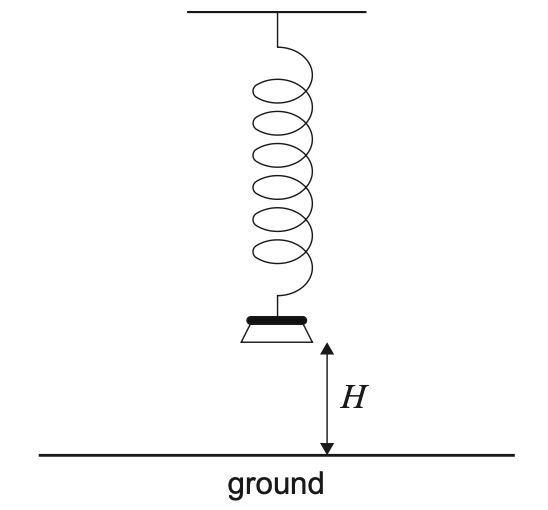
\includegraphics[width=0.30\textwidth]{../graphics/AA_SL_2023_May_P2_TZ2_Q08a_spring.png}
\end{center}

\begin{enumerate}[itemsep=0.05cm]
  \item Find the period of the function. \hfill [2]
\end{enumerate}

The weight is released when its base is at a minimum height of $1$ metre above the ground, and it reaches a maximum height of $1.8$ metres above the ground. The graph of $H$ is shown in the following diagram.

%\begin{center}
%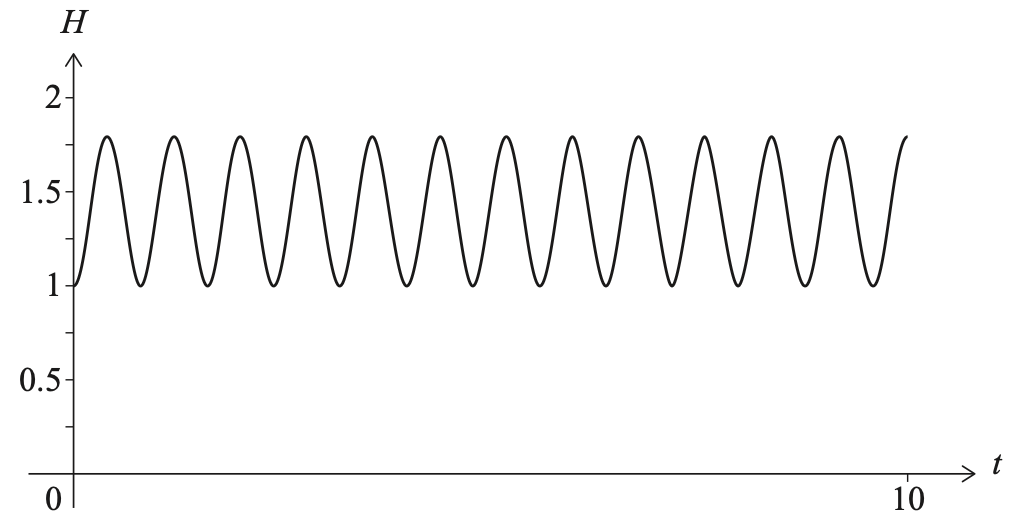
\includegraphics[width=0.50\textwidth]{../graphics/AA_SL_2023_May_P2_TZ2_Q08b_spring-graph.png}
%\end{center}

\begin{center}
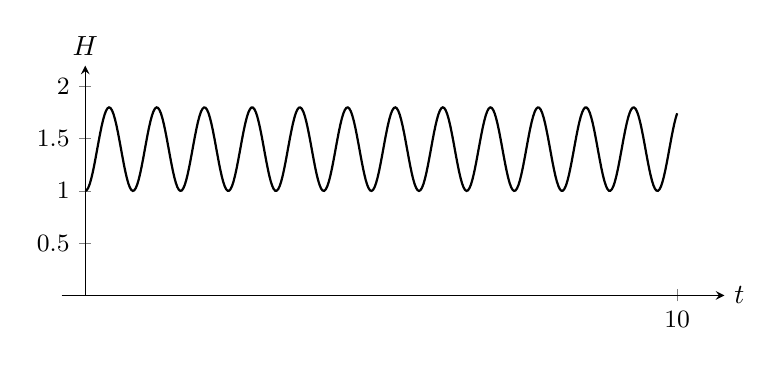
\begin{tikzpicture}
\begin{axis}[
    width=10cm, height=4.5cm,
    axis lines=middle,
    xlabel={$t$}, ylabel={$H$},
    xlabel style={at={(ticklabel* cs:1)}, anchor=west},
    ylabel style={at={(ticklabel* cs:1)}, anchor=south},
    xmin=-0.4, xmax=10.8,
    ymin=0, ymax=2.2,
    xtick={10}, xticklabels={10},
    ytick={0.5, 1, 1.5, 2},
    tick label style={font=\small},
    samples=400,
]
\addplot[thick, domain=0:10] {-0.4*cos(deg(7.8*x)) + 1.4};
\end{axis}
\end{tikzpicture}
\end{center}

\begin{enumerate}[itemsep=0.1cm]
  \item[(b)] Find the value of (i) $a$; (ii) $b$. \hfill [3]
  \item[(c)] Find the number of times that the weight reaches its maximum height in the first five seconds of its motion. \hfill [2]
  \item[(d)] Find the first time that the base of the weight reaches a height of $1.5$ metres. \hfill [2]
\end{enumerate}

A camera is set to take a picture of the weight at a random time during the first five seconds of its motion.

\begin{enumerate}[itemsep=0.1cm]
  \item[(e)] Find the probability that the height of the base of the weight is greater than $1.5$ metres at the time the picture is taken. \hfill [4]
\end{enumerate}

\newpage

%--- Problem 3: harbour tide [13 marks] ---
%--- Source: AA SL 2021 Nov P2 Q08 ---
%--- Answer on lined paper. ---
\item[3.] [Maximum mark: 13]

The height of water, in metres, in Dungeness harbour is modelled by the function
$$H(t) = a\sin(b(t - c)) + d,$$
where $t$ is the number of hours after midnight, and $a$, $b$, $c$, $d$ are constants with $a > 0$, $b > 0$ and $c > 0$.

The following graph shows the height of the water for 13 hours, starting at midnight.

%\begin{center}
%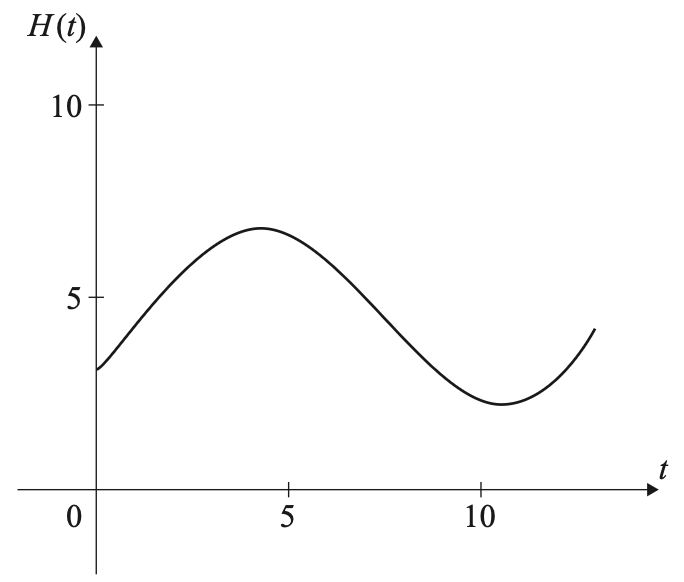
\includegraphics[width=0.5\textwidth]{../graphics/AA_SL_2021_Nov_P2_Q08_tide.png}
%\end{center}

\begin{center}
\begin{tikzpicture}
\begin{axis}[
    width=10cm, height=5cm,
    axis lines=middle,
    xlabel={$t$}, ylabel={$H(t)$},
    xlabel style={at={(ticklabel* cs:1)}, anchor=west},
    ylabel style={at={(ticklabel* cs:1)}, anchor=south},
    xmin=-0.5, xmax=14,
    ymin=0, ymax=10,
    xtick={5, 10}, ytick={5, 10},
    tick label style={font=\small},
    samples=300,
]
\addplot[thick, domain=0:13] {2.3*sin(deg((pi/6)*(x - 1.5))) + 4.5};
\end{axis}
\end{tikzpicture}
\end{center}

The first high tide occurs at 04:30 and the next high tide occurs $12$ hours later. Throughout the day, the height of the water fluctuates between $2.2$ m and $6.8$ m. All heights are given correct to one decimal place.

\begin{enumerate}[itemsep=0.1cm]
  \item Show that $b = \dfrac{\pi}{6}$. \hfill [1]
  \item Find the value of $a$. \hfill [2]
  \item Find the value of $d$. \hfill [2]
  \item Find the smallest possible value of $c$. \hfill [3]
  \item Find the height of the water at 12:00. \hfill [2]
  \item Determine the number of hours, over a 24-hour period, for which the tide is higher than $5$ metres. \hfill [3]
\end{enumerate}

\newpage

%--- Problem 4: windmill blade [13 marks] ---
%--- Source: AA SL 2021 May P2 TZ2 Q07 ---
%--- Answer on lined paper. ---
\item[4.] [Maximum mark: 13]

The six blades of a windmill rotate around a centre point $C$. Points $A$ and $B$ and the base of the windmill are on level ground, as shown in the following diagram.

\begin{center}
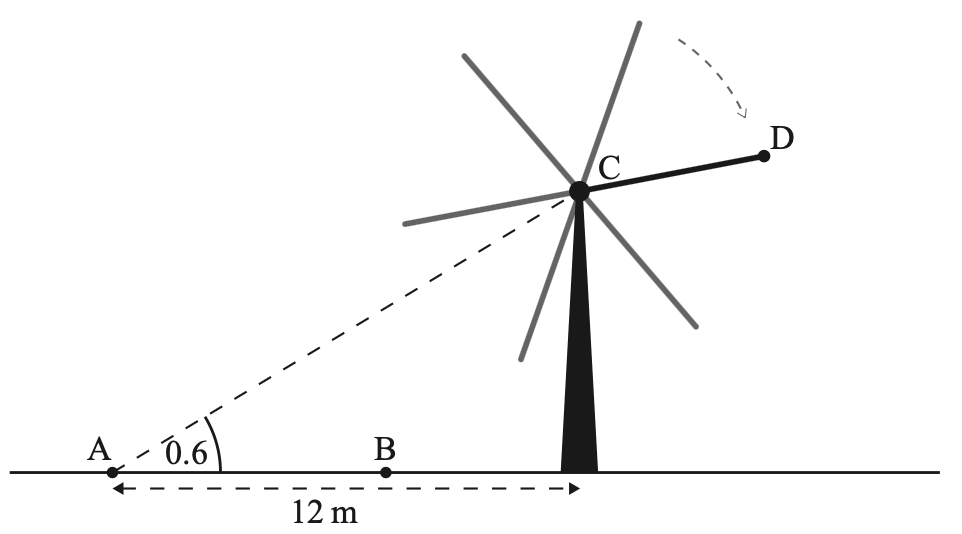
\includegraphics[width=0.65\textwidth]{../graphics/AA_SL_2021_May_P2_TZ2_Q07_windmill.png}
\end{center}

From point $A$ the angle of elevation of point $C$ is $0.6$ radians.

\begin{enumerate}[itemsep=0.1cm]
  \item Given that point $A$ is $12$ metres from the base of the windmill, find the height of point $C$ above the ground. \hfill [2]
\end{enumerate}

An observer walks $7$ metres from point $A$ to point $B$.

\begin{enumerate}[itemsep=0.1cm]
  \item[(b)] Find the angle of elevation of point $C$ from point $B$. \hfill [2]
\end{enumerate}

The observer keeps walking until he is standing directly under point $C$. The observer has a height of $1.8$ metres, and as the blades of the windmill rotate, the end of each blade passes $2.5$ metres over his head.

\begin{enumerate}[itemsep=0.1cm]
  \item[(c)] Find the length of each blade of the windmill. \hfill [2]
\end{enumerate}

One of the blades is painted a different colour than the others. The end of this blade is labelled point $D$. The height $h$, in metres, of point $D$ above the ground can be modelled by the function
$$h(t) = p\cos\!\left(\dfrac{3\pi}{10}\,t\right) + q,$$
where $t$ is in seconds and $p, q \in \mathbb{R}$. When $t = 0$, point $D$ is at its maximum height.

\begin{enumerate}[itemsep=0.1cm]
  \item[(d)] Find the value of $p$ and the value of $q$. \hfill [4]
\end{enumerate}

If the observer stands directly under point $C$ for one minute, point $D$ will pass over his head $n$ times.

\begin{enumerate}[itemsep=0.1cm]
  \item[(e)] Find the value of $n$. \hfill [3]
\end{enumerate}

\end{enumerate}
\end{document}
